\section{ハード構成}\label{ux30edux30dcux30c3ux30c8ux7af6ux6280ux5927ux4f1aux306eux6982ux8981}

ハード構成はFig.\ref{fig301}の通りです。
Fig.\ref{fig201}よりエンコーダを追加することで、モータの回転数を取得します。

\begin{itemize}
    \tightlist
    \item
    マイコン:Arduino Mega 2560 R3
    \item
    モータドライバ:VNH5019搭載モータードライバ (POLOLU-1451)
    \item
    モータ:75:1 シャフト付き超小型メタルギアドモーター HP (POLOLU-2215)
    \item
    エンコーダ:シャフト付き超小型メタルギアドモーター用磁気式エンコーダ (POLOLU-3081)
    \end{itemize}

\begin{figure}[htbp]
\centering
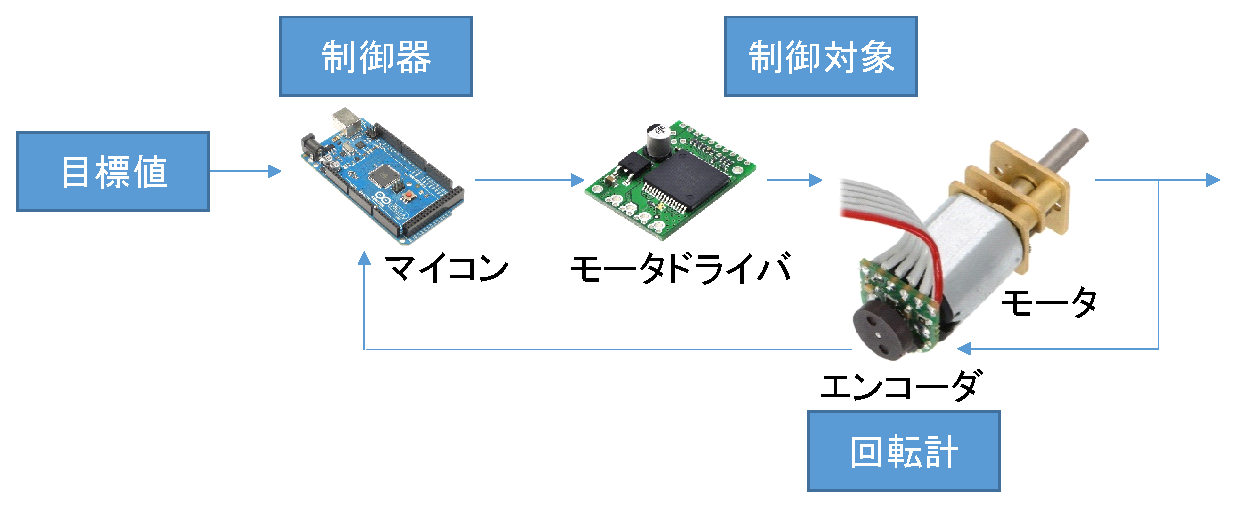
\includegraphics[width=300pt]{fig/fig301.eps}
\caption{ハード構成}
\label{fig301}
\end{figure}


\section{回路図}\label{ux69cbux60f3ux8a2dux8a08}

回路図はFig.\ref{fig302}の通りです。
Arduino Mega 2560 のピン2~3を使用してエンコーダ信号を読み取ります。
エンコーダの詳細は、Pololu HP \cite{pololu_HP_encoder} に記載されています。

\begin{figure}[htbp]
\centering
\includegraphics[width=380pt]{fig/fig302.eps}
\caption{回路図}
\label{fig302}
\end{figure}


\section{Simulinkモデル}\label{ux5168ux4f53ux69cbux6210}

Simulinkモデルは、Fig.\ref{fig303}の通りです。
エンコーダの出力信号を読み取るために、S-Function Builder ブロックを使用します。
ブロックの中身は、Fig.\ref{fig304}~Fig.\ref{fig307}の通りです。
それぞれのタブに設定を入れ、
"ライブラリ"タブの"インクルード"、"出力"タブ、"更新"タブに
Fig.\ref{fig308}~Fig.\ref{fig310}に示すプログラムを書き込んで、
"ビルド"を押すことでコンパイルができます。

プログラムは”離散状態の更新”でエンコーダに接続した割込みピンの設定を行い、
”インクルード”で呼び出し関数の定義を行い、
”出力”でプログラムをループさせ、
エンコーダ回転数[RPM]をS-Function Builder ブロックから出力させます。

\begin{figure}[htbp]
    \centering
    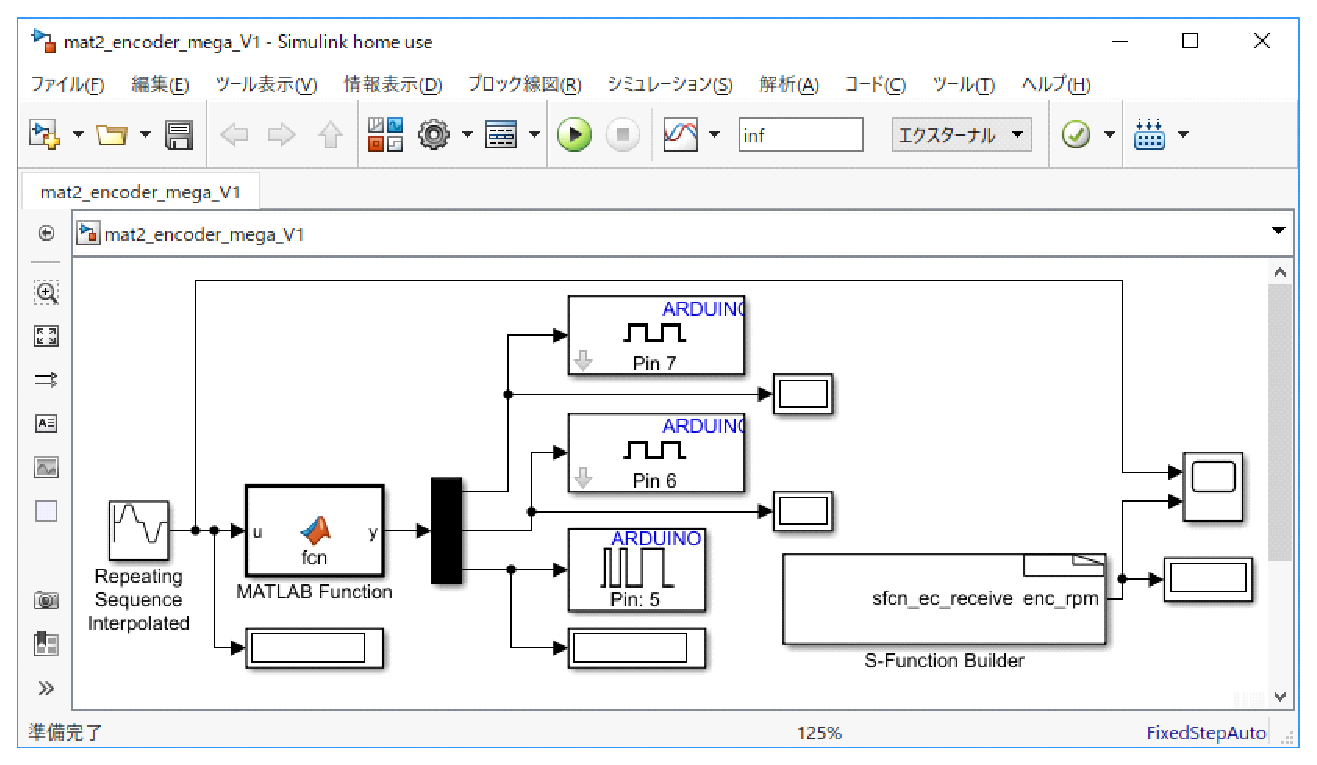
\includegraphics[width=380pt]{fig/fig303.eps}
    \caption{Matlab/Simulinkモデル}
    \label{fig303}
\end{figure}

\begin{figure}[htbp]
    \centering
    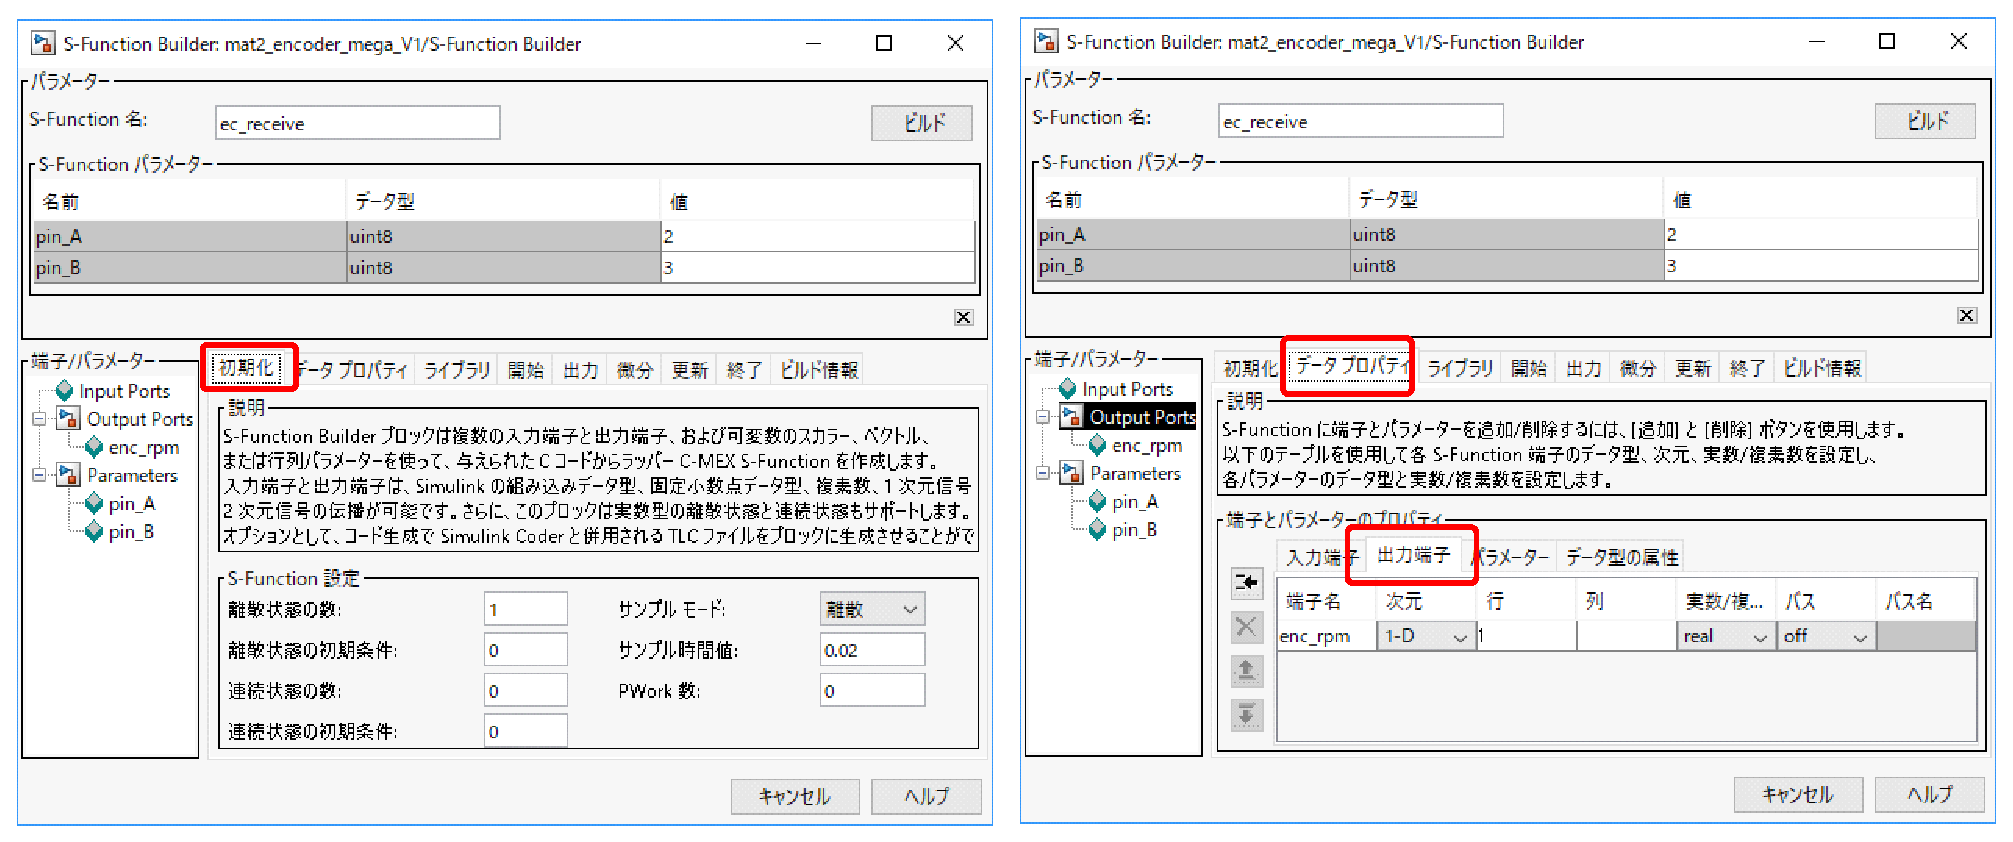
\includegraphics[width=380pt]{fig/fig304.eps}
    \caption{S-Function Builder}
    \label{fig304}
\end{figure}

\begin{figure}[htbp]
    \centering
    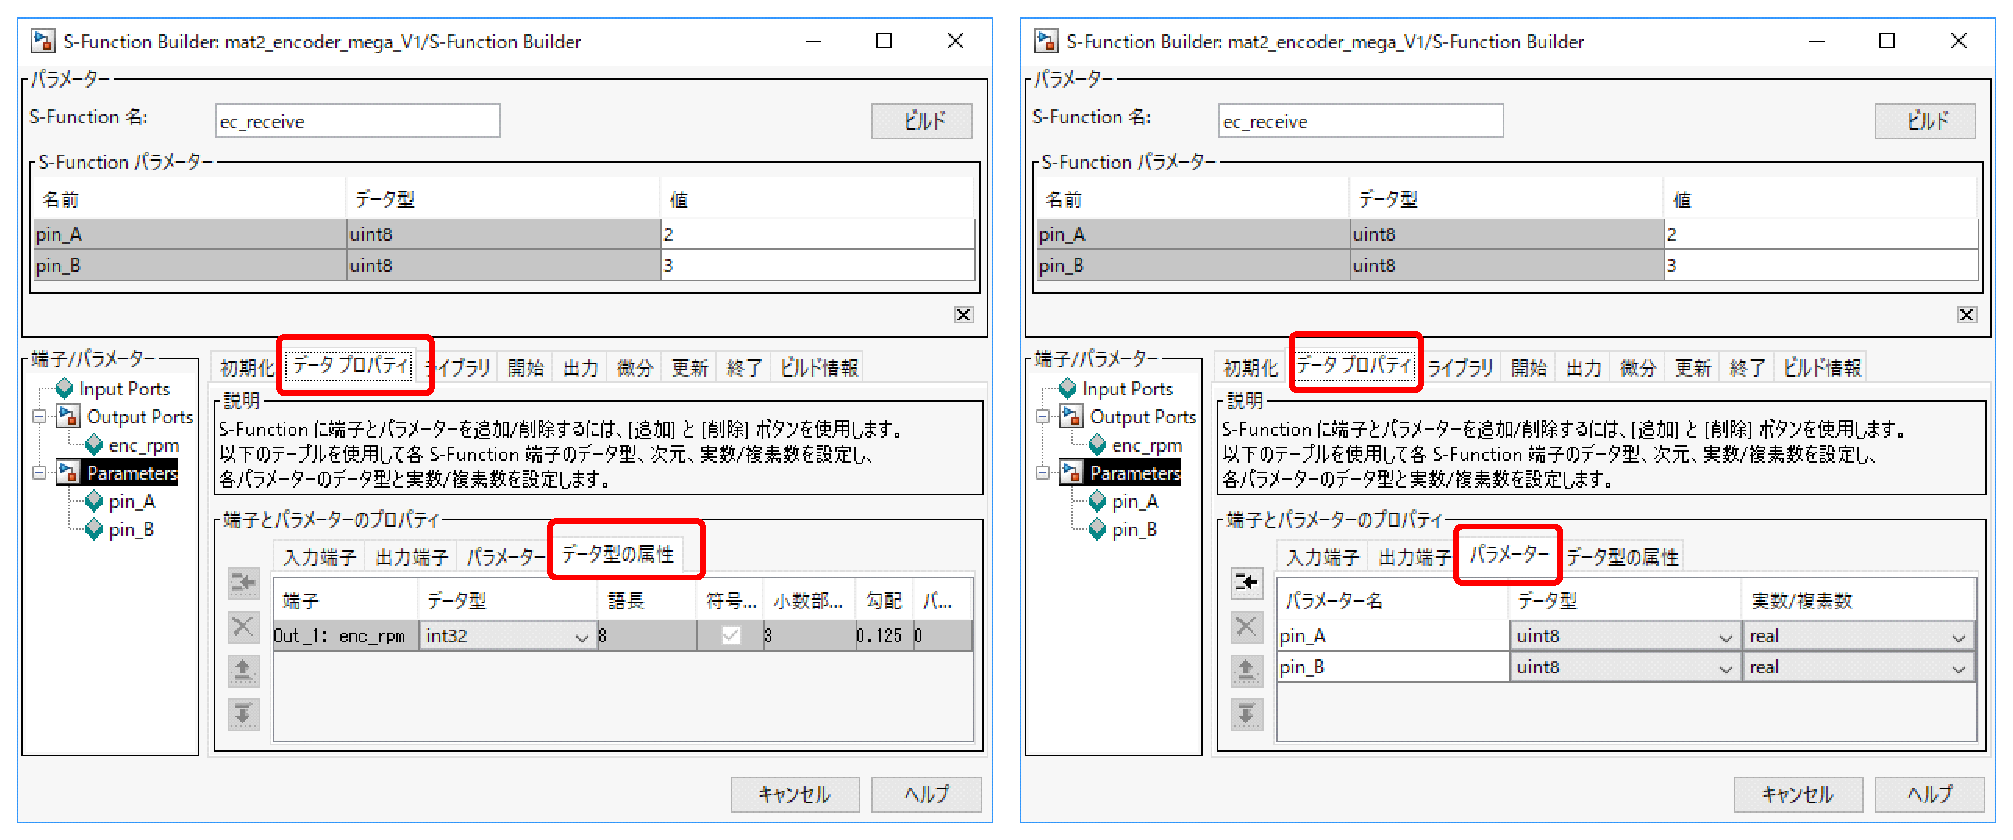
\includegraphics[width=380pt]{fig/fig305.eps}
    \caption{S-Function Builder}
    \label{fig305}
\end{figure}

\begin{figure}[htbp]
    \centering
    \includegraphics[width=380pt]{fig/fig306.eps}
    \caption{S-Function Builder}
    \label{fig306}
\end{figure}

\begin{figure}[htbp]
    \centering
    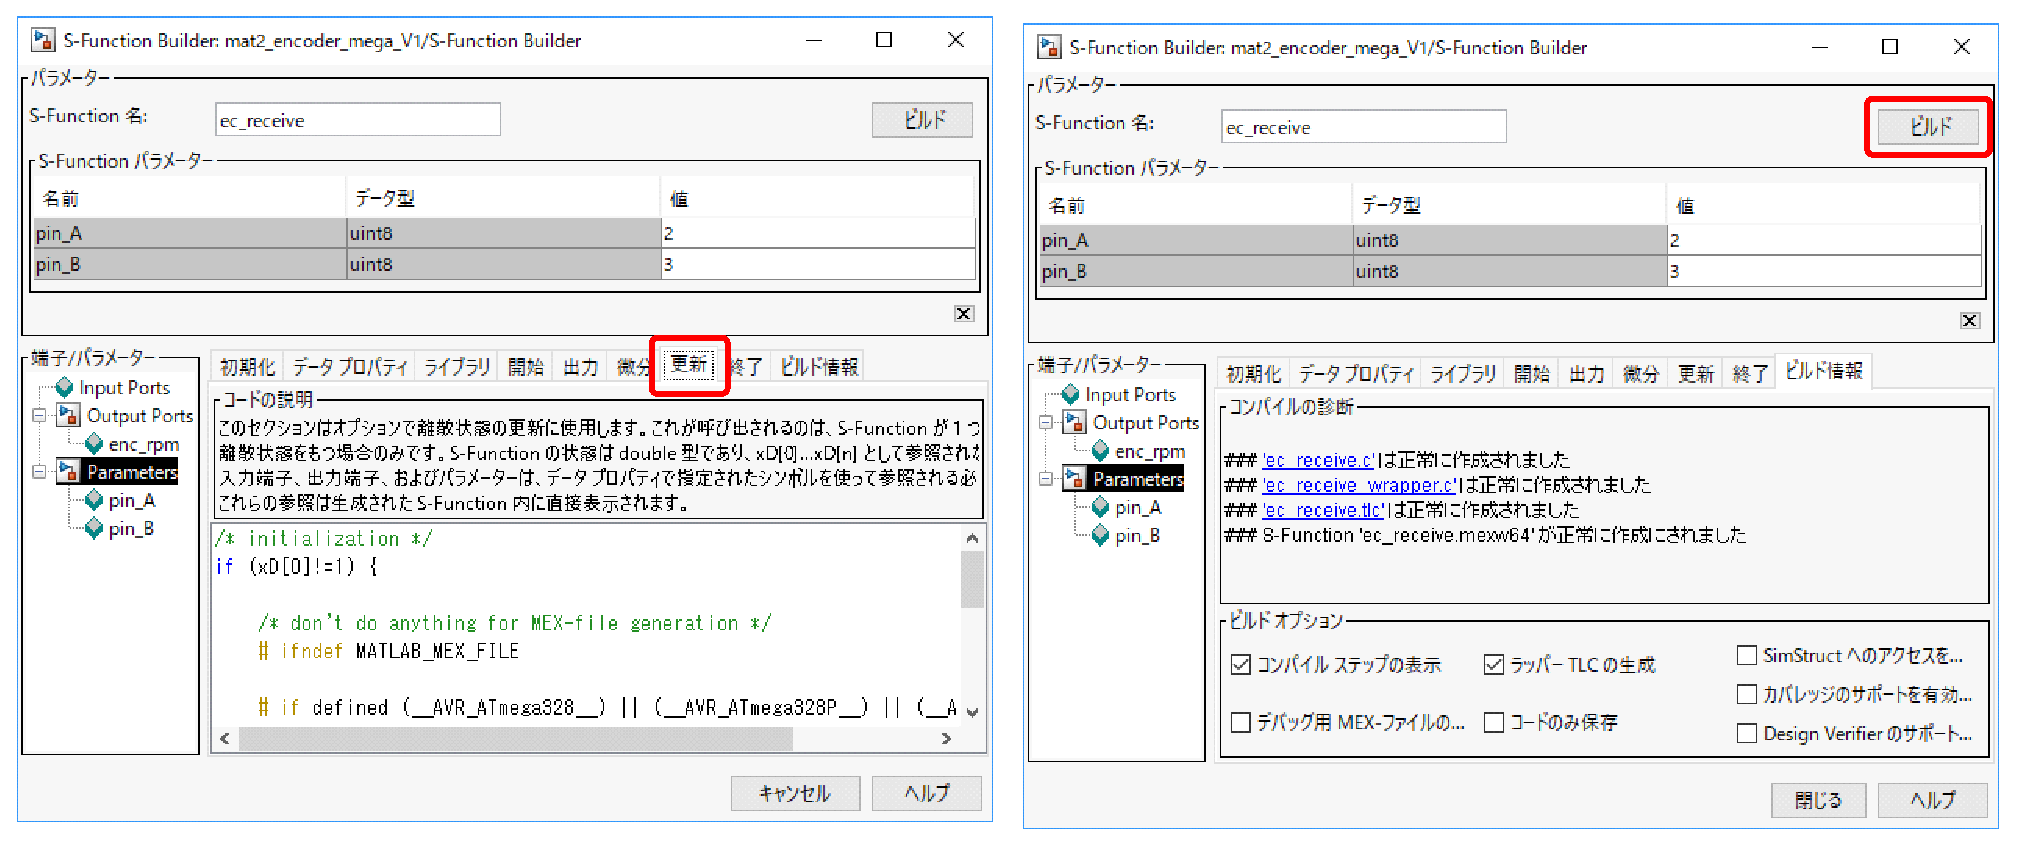
\includegraphics[width=380pt]{fig/fig307.eps}
    \caption{S-Function Builder}
    \label{fig307}
\end{figure}   

\begin{figure}[htbp]
    \centering
    \includegraphics[width=300pt]{fig/fig308.eps}
    \caption{S-Function Builder ライブラリ インクルード}
    \label{fig308}
\end{figure}   

\begin{figure}[htbp]
    \centering
    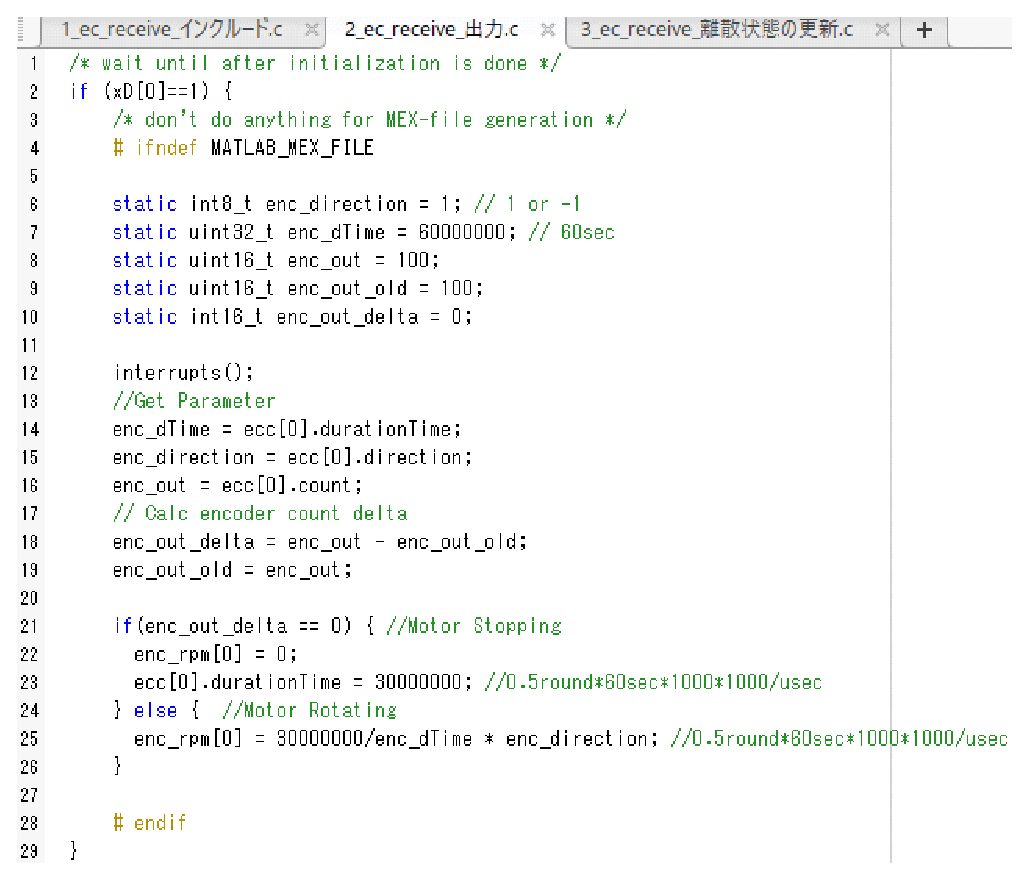
\includegraphics[width=320pt]{fig/fig309.eps}
    \caption{S-Function Builder 出力}
    \label{fig309}
\end{figure}  

\begin{figure}[htbp]
    \centering
    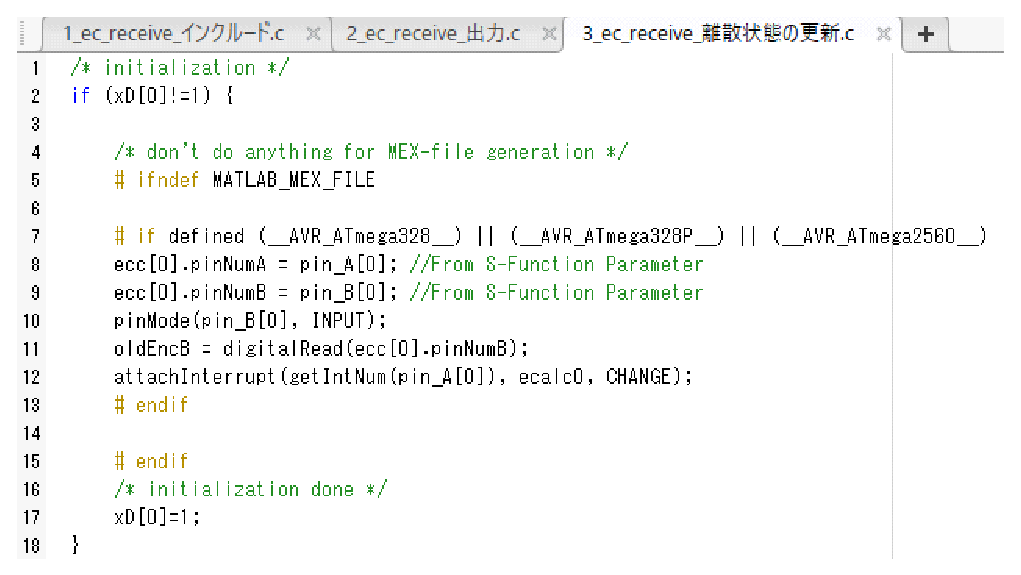
\includegraphics[width=320pt]{fig/fig310.eps}
    \caption{S-Function Builder 離散状態の更新}
    \label{fig310}
\end{figure}  


\clearpage
\section{実行}\label{ux811aux69cbux6210}

Scopeブロックのグラフ表示を立ち上げた状態で "実行" することで、
回転数測定結果をリアルタイムにグラフを描写できます。
実行例としてFig.\ref{fig311}に示します。
操作量に応じて、回転数が高くなることが確認できます。
\begin{figure}[htbp]
    \centering
    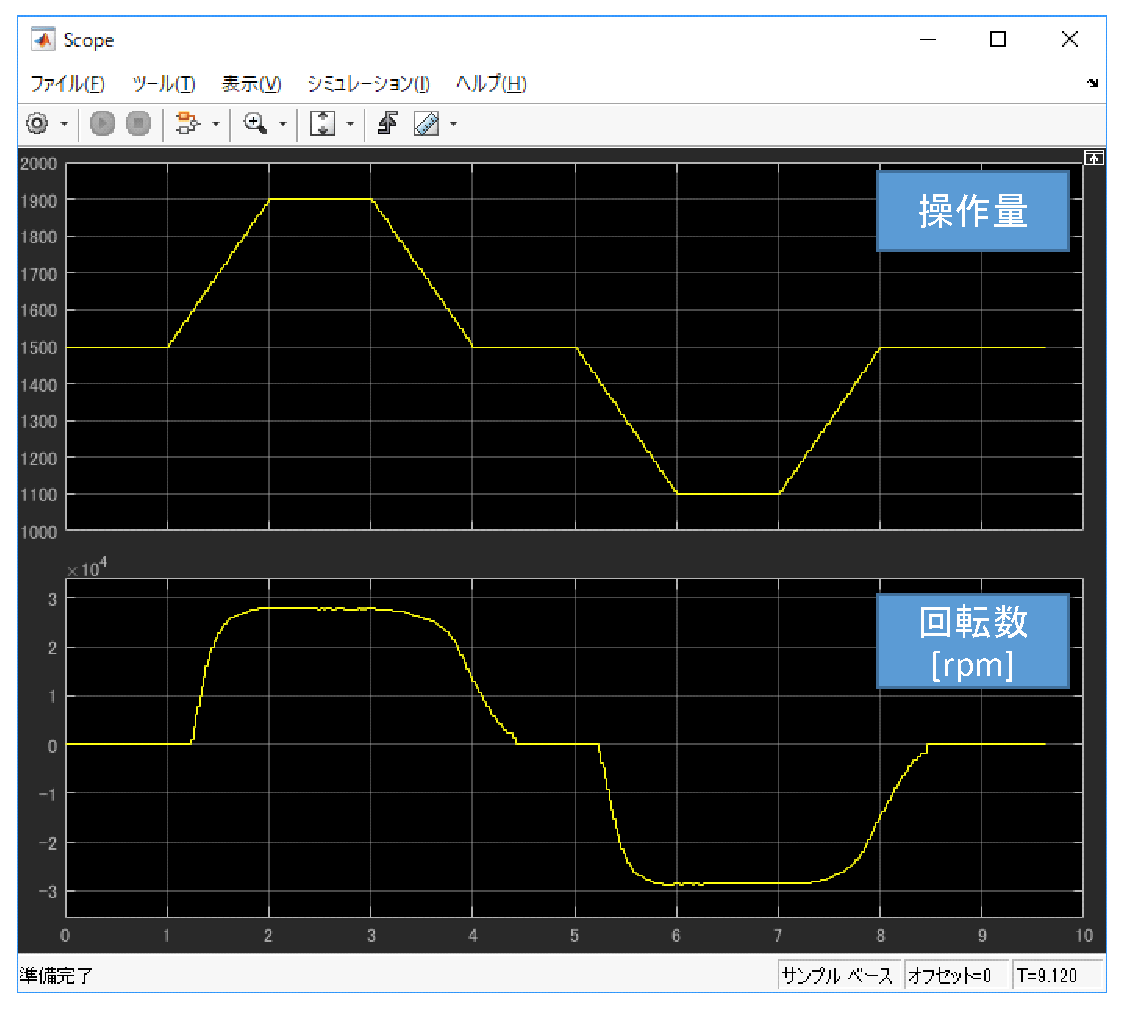
\includegraphics[width=200pt]{fig/fig311.eps}
    \caption{回転数の計測結果}
    \label{fig311}
\end{figure}

正しく回転数が計測できているか確認する方法として、
次のような外部計測器(Fig.\ref{fig312})を使う方法があります。
例えば回転計を使用する場合は、エンコーダの円盤に反射シールを張り付け、
モータを定常回転させれば回転数を計測できます。

\begin{itemize}
    \tightlist
    \item
    回転計:非接触デジタルタコメーター DT2234B
    \item
    オシロスコープ:MiniDSO DS203
    \end{itemize}

\begin{figure}[htbp]
    \centering
    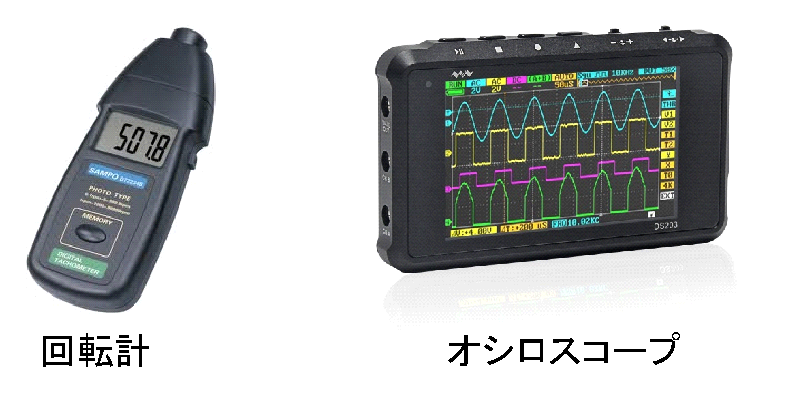
\includegraphics[width=200pt]{fig/fig312.eps}
    \caption{計測器}
    \label{fig312}
\end{figure}